\chapter{CAT(0)-Räume} % (fold)
\label{cha:1}

\begin{definition}[Metrischer Raum]
\label{def:1.1}
	Sei $X$ eine Menge.\marginnote{21.10.15 \\ \ [1]}
	Eine Abbildung $d \colon X \times X \rightarrow \RR_{\geq 0}$ heißt \Index{Metrik}, wenn für alle $x,y,z \in X$ gilt:
	\begin{enumerate}[(i)]
		\item $d(x,y) = 0 \Leftrightarrow x=y$
		\item $d(x,y) = d(y,x)$
		\item $d(x,z) \leq d(x,y) + d(y,z)$
	\end{enumerate}
	Das Paar $(X,d)$ heißt dann \Index{metrischer Raum}.
\end{definition}

\begin{beispiel}
\label{bsp:1.2}
	\mbox{} \\[-1.4cm]
	\begin{enumerate}[(i)]
		\item Für $n \in \NN$ ist $\EE^n := (\RR^n,d_2)$ mit
		\begin{align*}
			d_2\colon \RR^n \times \RR^n &\longrightarrow \RR_{\geq 0} \\
			(x,y) &\longmapsto \sqrt{\sum_{i=1}^{n} (x_i-y_i)^2}.
		\end{align*}
		\item Sei $X$ eine Menge.
		Wir definieren:
		\begin{align*}
			d\colon X \times X &\longrightarrow \RR_{\geq 0} \\
			(x,y) &\longmapsto \begin{dcases}
				1, & x \neq y \\
				0, & x = y.
			\end{dcases}
		\end{align*}
		Dann ist $d$ eine Metrik und $(X,d)$ heißt ein \textbf{diskreter metrischer Raum}. \index{metrischer Raum!diskret}
	\end{enumerate}
\end{beispiel}

\begin{definition}[Geodätischer Raum]
\label{def:1.3}
	\mbox{} \\[-1.4cm]
	\begin{enumerate}[(i)]
		\item Sei $(X,d)$ ein metrischer Raum und $x,y \in X$.
		Eine \Index{Geodäte} von $x$ nach $y$ ist eine Abbildung $\gamma \colon [a,b] \rightarrow X$ mit $\gamma(a) = x, \gamma(b) = y$ und $d(\gamma(t),\gamma(t')) = \abs{t-t'}$ für alle $t,t' \in [a,b]$.
		Wir schreiben $\gamma\colon x \geo y$.
		\item Der Raum $(X,d)$ ist ein \Index{geodätischer Raum}, wenn für alle $x,y \in X$ eine Geodäte $x \geo y$ existiert.
		\item Ein geodätischer Raum heißt \Index{eindeutig geodätisch}, wenn genau eine solche Geodäte existiert.
	\end{enumerate}
\end{definition}
\newpage
\begin{beispiel}
\label{bsp:1.4}
	\mbox{} \\[-1.4cm]
	\begin{enumerate}[(i)]
		\item Sei $(V, \Norm{\cdot})$ ein normierter reeller Vektorraum.
		Dann ist $(V,d_{\Norm{\cdot}})$ ein geodätischer Raum.
		Im Detail:
		Seien $u,v \in V$ paarweise verschieden und $L := \Norm{u-v} \neq 0$.
		Dann ist
		\begin{align*}
			\gamma\colon [0,L] &\longrightarrow V \\
			t &\longmapsto \enbrace*{1- \frac{t}{L}}\cdot u + \frac{t}{L} \cdot v
		\end{align*}
		eine Geodäte von $u$ nach $v$.
		\item $(\RR^2 \setminus \setzero, d_2)$ ist nicht geodätisch:
		Es existiert keine Geodäte $(-1,0) \geo (1,0)$.
		\item $(\RR^2,d_1)$ ist geodätisch, aber nicht eindeutig geodätisch:
		In der folgenden Abbildung sind zwei Geodäten von $(1,0) \geo (0,1)$ dargestellt.
		\begin{figure}[h]
		\centering
		\begin{tikzpicture}[scale=3,{>=Latex[]}]
			\draw[->] (-.2,0) -- (1.2,0);
			\draw[->] (0,-.2) -- (0,1.2);
			\draw (0,0) node[anchor=north east]{$0$};
			\draw (1,0.1) -- (1,-.1) node[below]{$1$};
			\draw (.1,1) -- (-.1,1) node[left]{$1$};
			
			\draw[->,very thick,color=red] (1,0) -- (0,1);
			\draw[->,very thick,color=blue] (1,.01) -- (.01,.01) -- (.01,1);
		\end{tikzpicture}
		\caption{Der metrische Raum $(\RR^2,d_1)$ ist nicht eindeutig geodätisch.}
		\end{figure}
	\end{enumerate}
\end{beispiel}

\begin{definition}[Geodätisches Dreieck]
\label{def:1.5}
	Ein \Index{geodätisches Dreieck} $\Delta = \Delta(x,y,z,\alpha,\beta,\gamma)$ in einem geodätischen Raum $(X,d)$ ist gegeben durch ein Tripel $(x,y,z) \in X^3$ und Geodäten $\alpha \colon x \geo y$, $\beta\colon y \geo z$, $\gamma \colon z \geo x$ -- den Seiten von $\Delta$.
\end{definition}

\begin{beispiel}
\label{bsp:1.6}
	\mbox{} \\[-1cm]
	\begin{figure}[h]
		\centering
		\begin{tikzpicture}[scale=2.5,>=Latex]
		\draw (-1,1) node[right]{$(\RR^2,d_1)$};
		\draw[->] (-1.1,0) -- (1.2,0);
		\draw[->] (0,-.3) -- (0,1.2);
		\draw (-1,.1) -- (-1,-.1) node[below]{$-1$};
		\draw (1,.1) -- (1,-.1) node[below]{$1$};
		\draw (-.1,1) -- (.1,1) node[right]{$1$};
		\draw[->,very thick, color=blue] (-1,0.02) -- (-0.02,0.02) -- (-0.02,1);
		\draw[->,very thick, color=red] (0.02,1) -- (0.02,0.02) -- (1,0.02);
		\draw[->,very thick, color=SeaGreen4] (1,-0.02) -- (-1,-0.02);
		\end{tikzpicture} \hspace{2cm}
		\begin{tikzpicture}[scale=2.5,>=Latex]
			\draw (-1,1) node[right]{$(\RR^2,d_1)$};
			\draw[->] (-1.1,0) -- (1.2,0);
			\draw[->] (0,-.3) -- (0,1.2);
			\draw (-1,.1) -- (-1,-.1) node[below]{$-1$};
			\draw (1,.1) -- (1,-.1) node[below]{$1$};
			\draw (-.1,1) -- (.1,1) node[right]{$1$};
			
		\draw[->,very thick, color=blue] (-1,0) -- (0,1);
		\draw[->,very thick, color=red] (0,1) -- (1,0);
		\draw[->,very thick, color=SeaGreen4] (1,0.02) -- (-1,0.02);
		\end{tikzpicture}
		\caption{Geodätische Dreiecke sind im Allgemeinen durch ihre Ecken nicht eindeutig bestimmt.}
	\end{figure}
\end{beispiel}

Die Dreiecksungleichung garantiert, dass es Punkte $\ol{x},\ol{y},\ol{z} \in \EE^2$ gibt mit $d(x,y) = d_2(\ol{x},\ol{y})$, $d(y,z) = d_2(\ol{y},\ol{z})$, $d(z,x) = d_2(\ol{z},\ol{x})$ und Geodäten
\[
	\ol{\alpha}(t) = \ol{x} + t \cdot \frac{\ol{y}-\ol{x}}{d_2(\ol{y},\ol{x})}, \quad \ol{\beta}(t) = \ol{y} + t \cdot \frac{\ol{z}-\ol{y}}{d_2(\ol{z},\ol{y})}, \quad
	\ol{\gamma}(t) = \ol{z} + t \cdot \frac{\ol{x}-\ol{z}}{d_2(\ol{x},\ol{z})}.
\]
$\ol{\Delta} = \ol{\Delta}(\ol{x},\ol{y},\ol{z},\ol{\alpha},\ol{\beta},\ol{\gamma})$ heißt \Index{Vergleichsdreieck} zu $\Delta(x,y,z,\alpha,\beta,\gamma)$.
Ist $v = \gamma(s)$ für ein $s$, so heißt $\ol{v} = \ol{\gamma}(s)$ \Index{Vergleichspunkt} von $v$.

\begin{definition}[$\CAT$-Raum]
\label{def:1.7}
	\mbox{} \\[-1.4cm]
	\begin{enumerate}[(i)]
		\item Ein Dreieck $\Delta$ in $(X,d)$ hat die \textbf{CAT(0)-Eigenschaft}, wenn für alle $n,m$ auf den Seiten von $\Delta$ und ihre Vergleichspunkte $\ol{n},\ol{m}$ auf den Seiten von $\ol{\Delta}$. \index{CAT(0)-Raum@$\CAT$-Raum}
		\item Ein metrischer Raum $(X,d)$ ist ein \textbf{CAT(0)-Raum}, wenn $(X,d)$ geodätisch ist und alle seine Dreiecke die $\CAT$-Eigenschaft erfüllen.
		\item Ein metrischer Raum $(X,d)$ heißt \textbf{lokal CAT(0)}, wenn für alle $x \in X$ ein $r_x > 0$ existiert, sodass
		\[
			B_{r_x}(x) = \{y \in X : d(y,x) < r_x\}
		\]
		mit der induzierten Metrik ein $\CAT$-Raum ist. \index{CAT(0)-Raum@$\CAT$-Raum!lokal}
	\end{enumerate}
\end{definition}

\begin{figure}[h]
	\centering
	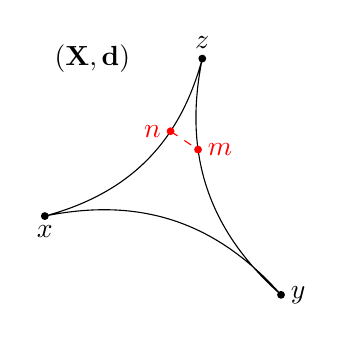
\begin{tikzpicture}[scale=1]
	\draw (0,1) node[fill,circle,inner sep=1pt]{}
	to [bend left] (3,0) node[fill,circle,inner sep=1pt]{} 
	to [bend left] coordinate[pos=.66] (M) (2,3) node[fill,circle,inner sep=1pt]{}
	to [bend left] coordinate[pos=.33] (N) cycle;
	\draw (0,1) node[below]{$x$};
	\draw (3,0) node[right]{$y$};
	\draw (2,3) node[above]{$z$};
	\draw (N) node[fill,circle,inner sep=1pt,color=red]{};
	\draw (N) node[left,color=red]{$n$};
	\draw (M) node[fill,circle,inner sep=1pt,color=red]{};
	\draw (M) node[right,color=red]{$m$};
	\draw[color=red, dashed] (N) -- (M);
	\draw (0,3) node[right]{$\mathbf{(X,d)}$};
	\end{tikzpicture} \hspace{2cm}
	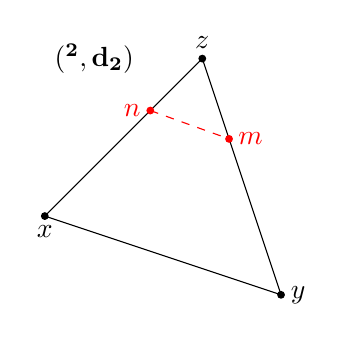
\begin{tikzpicture}[scale=1]
	\draw (0,1) node[fill,circle,inner sep=1pt]{}
	to (3,0) node[fill,circle,inner sep=1pt]{} 
	to coordinate[pos=.66] (M) (2,3) node[fill,circle,inner sep=1pt]{}
	to coordinate[pos=.33] (N) cycle;
	\draw (0,1) node[below]{$\ol{x}$};
	\draw (3,0) node[right]{$\ol{y}$};
	\draw (2,3) node[above]{$\ol{z}$};
	\draw (N) node[fill,circle,inner sep=1pt,color=red]{};
	\draw (N) node[left,color=red]{$\ol{n}$};
	\draw (M) node[fill,circle,inner sep=1pt,color=red]{};
	\draw (M) node[right,color=red,xshift=-.2]{$\ol{m}$};
	\draw[color=red, dashed] (N) -- (M);
	\draw (0,3) node[right]{$\mathbf{(\RR^2,d_2)}$};
	\end{tikzpicture}	
	\caption{Anschaulich gesprochen sind Dreiecke in $\CAT$-Räumen \enquote{mindestens so dünn} wie ihre Vergleichsdreiecke im euklidischen Raum.}
\end{figure}

\begin{bemerkung}
\label{bem:1.8}
	\mbox{} \\[-1.4cm]
	\begin{enumerate}[(i)]
		\item Lokal $\CAT$-Räume heißen auch nichtpositiv gekrümmte oder Alexandrov-Räume.
		\item $\CAT$ steht für \textsc{Cartan-Alexandrov-Topogonov} und Krümmung $\leq 0$.
	\end{enumerate}
\end{bemerkung}

\begin{beispiel}
\label{bsp:1.9}
	\mbox{} \\[-1.4cm]
	\begin{enumerate}[(i)]
		\item Der euklidische Raum $\EE^n$ ist $\CAT$.
		\item $(\RR^2,d_1)$ ist nicht $\CAT$: In der folgenden Abbildung~\ref{abb:1.4} ist $d_1(n,m) = 2$, aber $d_2(\ol{n},\ol{m}) = \sqrt{3}$.
		\begin{figure}[h]
			\centering
			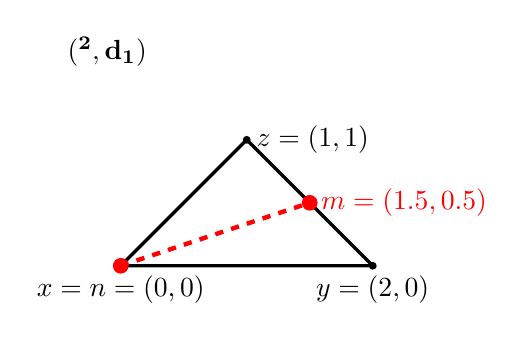
\begin{tikzpicture}[scale=1.6]	
			\draw (-1,0) node[below]{$x = n = (0,0)$};
			\draw (1,0) node[below]{$y = (2,0)$};
			\draw (0,1) node[right]{$z = (1,1)$};
			
			\draw[very thick] (-1,0) node[fill,circle,inner sep=2pt,color=red]{} -- (1,0) node[fill,circle,inner sep=1pt]{} -- coordinate[pos=.5] (M) (0,1) node[fill,circle,inner sep=1pt]{} -- cycle;
			
			\draw (M) node[fill,circle,inner sep=2pt,color=red]{};
			\draw (M) node[right,color=red,xshift=.6]{$m = (1.5,0.5)$};
			\draw[color=red,dashed,ultra thick] (-1,0) -- (M);
			\draw (-1.5,1.7) node[right]{$\mathbf{(\RR^2,d_1)}$};
			\end{tikzpicture} \hspace{1.5cm}
			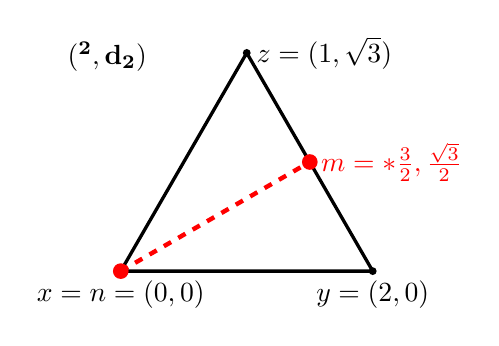
\begin{tikzpicture}[scale=1.6]	
			\draw[very thick] (0,0) node[fill,circle,inner sep=2pt,color=red]{} -- (2,0) node[fill,circle,inner sep=1pt]{} -- coordinate[pos=.5] (M) (1,1.732051) node[fill,circle,inner sep=1pt]{} -- cycle;
			
			\draw (0,0) node[below]{$\ol{x} = \ol{n} =(0,0)$};
			\draw (2,0) node[below]{$\ol{y} = (2,0)$};
			\draw (1,1.732051) node[right]{$\ol{z} = (1,\sqrt{3})$};
			
			\draw (M) node[fill,circle,inner sep=2pt,color=red]{};
			\draw (M) node[right,color=red,xshift=.6]{$\ol{m} = \enbrace*{\frac{3}{2},\frac{\sqrt{3}}{2}}$};
			\draw[color=red,dashed,ultra thick] (0,0) -- (M);
			\draw (-0.5,1.7) node[right]{$\mathbf{(\RR^2,d_2)}$};	
			\end{tikzpicture}
			\caption{Der Raum $(\RR^2,d_1)$ ist nicht $\CAT$.}
			\label{abb:1.4}
		\end{figure}
		\item Hilberträume sind $\CAT$.
		\item Komplemente von Polygonen im $\RR^2$ sind lokal $\CAT$, aber nicht $\CAT$.	
	\end{enumerate}
\end{beispiel}

\begin{beobachtung}
\label{beob:1.10}
	Sei $(X,d)$ ein $\CAT$-Raum.
	Dann ist $X$ eindeutig geodätisch.
\end{beobachtung}

\begin{beweis}
	Seien $\gamma\colon x \geo y$ und $\gamma'\colon x \geo y$ zwei Geodäten von $x$ nach $y$.
	Seien $p$ und $p'$ zwei Punkte auf $\gamma$ und $\gamma'$ mit $d(x,p) = d(x,p')$.
	Das Vergleichsdreieck $\ol{\Delta}$ zum Dreieck
	\[
		\Delta = \Delta(x,p,y\gamma \big|_{[0,d(x,p)]}, \gamma \big|_{[d(x,p),d(x,y)]},\gamma')
	\]
	ist degeneriert:
	\begin{figure}[h]
		\centering
		\begin{tikzpicture}[scale=1.5,>=Latex]
			\draw (0,0) node[fill,circle,inner sep=1.5pt,color=black]{};
			\draw (3,0) node[fill,circle,inner sep=1.5pt,color=black]{};
			\draw [->,very thick,color=red] (0,0) to [bend left] coordinate[pos=0.3] (P) (3,0);
			\draw [->,very thick,color=blue] (0,0) to [bend right] coordinate[pos=0.3] (Q) (3,0);
			
			\draw (0,0) node[left]{$x$};
			\draw (3,0) node[right]{$y$};
			
			\draw (P) node[fill,circle,inner sep=1.5pt,color=black]{};
			\draw (Q) node[fill,circle,inner sep=1.5pt,color=black]{};
			\draw (P) node[above]{$p$};
			\draw (Q) node[below]{$p'$};
			
			\draw[color=red] (1.5,.5) node[above]{$\gamma$};
			\draw[color=blue] (1.5,-.5) node[below]{$\gamma'$};
		\end{tikzpicture} \hspace{2cm}
		\begin{tikzpicture}[scale=1.5,>=Latex]
		\draw (0,0) node[fill,circle,inner sep=1.5pt,color=black]{};
		\draw (3,0) node[fill,circle,inner sep=1.5pt,color=black]{};
		\draw [->,very thick,color=red] (0,0.01) to coordinate[pos=0.3] (P) (3,0.01);
		\draw [->,very thick,color=blue] (0,-0.01) to  coordinate[pos=0.3] (Q) (3,-0.01);
		
		\draw (0,0) node[left]{$\ol{x}$};
		\draw (3,0) node[right]{$\ol{y}$};
		
		\draw (P) node[fill,circle,inner sep=1.5pt,color=black]{};
		\draw (Q) node[fill,circle,inner sep=1.5pt,color=black]{};
		\draw (P) node[above]{$\ol{p}$};
		\draw (Q) node[below]{$\ol{p'}$};
		
		\draw[color=red] (1.5,.1) node[above]{$\ol{\gamma}$};
		\draw[color=blue] (1.5,-.1) node[below]{$\ol{\gamma'}$};
		\end{tikzpicture}
	\end{figure}
	
	Wegen der $\CAT$-Eigenschaft gilt $d(p,p') \leq d(\ol{p},\ol{p'}) = 0$, also folgt $d(p,p')=0$ und $p = p'$.
\end{beweis}

\begin{definition}[Konvexe Menge]
\label{def:1.11}
	Sei $X$ ein $\CAT$-Raum. Eine nichtleere Teilmenge $C \subseteq X$ heißt \Index{konvex}, wenn zu allen $p,q \in C$ die Geodäte $\gamma \colon p \geo q$ in $C$ liegt.
\end{definition}

Offensichtlich ist $C$ wieder ein $\CAT$-Raum und Durchschnitte konvexer Mengen sind wieder konvex.
\cleardoubleoddemptypage